
Mediante este ensayo, se pretende calcular el valor de la potencia eficaz máxima de salida del amplificador, tanto a lazo abierto, como cerrado. Para llegar a esto, se medirá la tensión de salida máxima del amplificador (sin distorciones), con una resistencia de carga igual a la impedancia de salida obtenida en la sección anterior ($R_o$, para lazo abierto y $R_o'$, para lazo cerrado) y en base a eso, mediante una fórmula se calculará la potencia máxima de salida. 

Los fundamentos de este experimento se encuentran en la sub-sección \ref{sec:MaxPot}, del Marco Teórico.

%\subsubsection{Fundamento}

\subsubsection{Implementación y Mediciones}

Se empleará el mismo circuito amplificador que en el experimento anterior (\ref{fig:esq_amp_tp3}), pero conectado de la siguiente manera (figura \ref{fig:circ6}):

\begin{figure}[H]
    \centering
    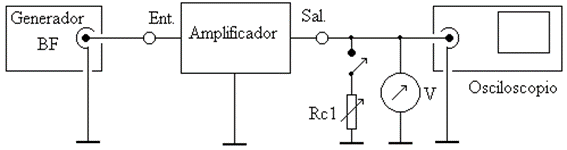
\includegraphics[width=0.85\textwidth]{Imagenes/circ6.png}
    \caption{Diagrama del circuito a ensayar}
    \label{fig:circ6}
\end{figure}

Como se explicó, la resistencia de carga $R_{C1}$ deberá ser igual a $R_o$ para lazo abierto. Revisando el circuito en la figura \ref{fig:esq2_amp_tp3}, se ve que colocando un jumper en la posición \textit{JS4}, se coloca como resistencia de carga una resistencia de 560 $\Omega$, muy similar a $R_o$. 

Una vez allí, se configura la frecuencia del generador a 1 kHz y se varía la amplitud hasta obtener la máxima salida antes de que recorte. En este caso el valor de tensión obtenido fue de 4,2 $V_{pp}$. 

Ahora se repetirá el mismo procedimiento pero para el amplificador realimentado (lazo cerrado), y cambiando el jumper de a la posición \textit{JS1}, haciendo que ahora la resistencia de carga $R_{C1}$ sea de 33 $\Omega$, un valor bastante próximo al de $R_o'$. En este caso, la tensión máxima de salida fue de 508 $mV_{pp}$.


\subsubsection{Cálculos}

Finalmente para calcular la potencia máxima de transferencia de nuestro amplificador, se empleará la siguiente fórmula (ecuación \ref{eq:potmax}):

\begin{equation}
    P_{max} = \cfrac{V_{rms}^2}{R} = \cfrac{V_{pp}^2}{8R}
    \label{eq:potmax}
\end{equation}

Obteniendo los siguientes valores como resultado (tabla \ref{tab:exp6}):

\begin{table}[H]
    \centering
    \scalebox{1}{
    \begin{tabular}{|c|c|c|}
    \hline
          & Lazo abierto & Lazo cerrado \\
          & ($R_{C1}=R_o$) & ($R_{C1}=R_o'$) \\
    \hline
        P [mW]  & 3.938 & 0.978 \\
    \hline
        \end{tabular}}
        \def\tablename{Tabla} 
        \caption{Potencias calculadas}
        \label{tab:exp6}
\end{table}
